\documentclass[../main.tex]{subfiles}

\begin{document}

\chapter{The Analytical Method}
\label{dts:chapter:intro}

For Phase-2, present DT on-detector electronics will be replaced by new boards, the so-called OBDT, which will perform the time digitisation of the chamber signals inside radiation-tolerant FPGAs with a time bin of 0.78~ns (25/32~ns) and a dead time of 100 ns as a result of the minimum DT front-end board deadtime. This time resolution is the same that is being used at present in the DT readout system and therefore, in the offline reconstruction. However, the legacy trigger system needed to work with lower resolution sampling of 12.5~ns and dead times of 400~ns. During Phase-2, all the incoming chamber signals will be sent asynchronously streamed via high-speed optical links to the back-end system, outside the experimental cavern, where the trigger primitives are generated in commercial FPGAs. 

In order to implement a new algorithm for trigger primitive generation during HL-LHC, several concerns exist and need to be addressed.
\begin{itemize}
	\item When a new LHC orbit starts, during the first bunch crossing (BX0), all counters used as a reference for the time of the hits in the DT cells are reset. Then, a hit timestamp ($t_{\text{TDC}}$) can be split in several contributions:
	\begin{equation}
		t_{\text{TDC}} = t_0 + t_{\text{TOF}} + t_e + t_d,
	\end{equation}
	where $t_0$ is the time difference between the BX0 and the BX of the collision that produced the muon, $t_{\text{TOF}}$ is the time of flight of the muon, $t_e$ is the sum of all processing times coming from the electronics involved, and $t_d$ is the drift time from the ionized electrons, which depends on where the muon crossed the DT cell. $t_{\text{TOF}}$ and $t_e$ can be determined per cell by calibrating the detector, although they introduce an uncertainty on the value of $t_{\text{TDC}}$. Both $t_d$ and $t_{\text{TDC}}$ need to be determined when generating the trigger primitives, taking into account a collision is produced every 25~ns and the maximum drift time is $\sim400$~ns, so a signal could be produced by the sixteen previous collisions.
	\item The timing information from the hits is not intrinsic to the time of the arrival of the hit timestamps, as it was in the Phase-1 system. Therefore, the new algorithm must be capable of sorting the hits and cope with a longer buffering time to ensure that all the relevant information is available before generating the trigger primitive.
	\item Since the dead time is reduced from 400~ns to approximately 100~ns, the number of hits in the same cell that could potentially belong to the same muon can increase by a factor 4, increasing the possible combinations of hits from different layers exponentially.
	\item The ageing of the chamber due to accumulated charge, as a consequence of the increased radiation, will reduce the efficiency of each DT cell. Accordingly, the DT trigger has to allow low quality combinations to account for this drop in efficiency in order to guarantee a fully efficient muon measurement.
	\item The increased PU during HL-LHC leads to a higher activity in the detector, increasing the hit rate in the DT chambers.
\end{itemize}

In summary, an algorithm with the capabilities of the offline reconstruction algorithm but in real time and handling hits with unknown arrival times had to be implemented. It is to be noted that the actual algorithm, without the HL-LHC added requirements, is already quite complex since it requires to perform a fit of the hits positions with the added unknown of the hits laterality (left or right to the wire) and the hits arrival time.

The \textit{Analytical Method} (AM) \cite{dts:intro:am} is the algorithm developed for performing muon trigger primitive (TP) generation for Phase-2 in the CMS barrel by using information from the DT system. It profits from the improved time digitization at trigger level in Phase-2 DT input hits, 25/32 ns ($\equiv1$~\textit{TDC count}), much finer than the 25~ns needed for bunch crossing (BX) identification. The input information to the AM algorithm is the wire numbers of the hit cells and the corresponding hit times with respect to the start of the LHC orbit. From these, using the known value of the drift velocity, and assuming a given laterality hypothesis (whether the signal was produced right or left of the cell wire), the hit position is reconstructed. For a given hypothesis of muon trajectory within a given chamber, by assuming it is a straight segment, the collision time, local direction and local position can be analytically determined, with a resolution comparable to what is reachable with the present offline reconstruction software \cite{intro:id:muon_7tev}.

A brief description of the algorithm and its performance results were recently published in Ref.~\cite{dts:intro:am}. In this chapter, the latest version of the algorithm will be presented. Section~\ref{sec:dts:description} includes a detailed description of the algorithm. Section~\ref{dts:sec:performance} shows its performance results using simulated events, while Section~\ref{hh:sec:fw} and \ref{hh:sec:st} describe studies performed with the software emulator and the firmware implementation in the laboratory and in the CMS DT Slice Test.

I have been involved in the development of the new trigger algorithm during the whole length of my thesis. I started as one of the developers of the first version of the algorithm, being the responsible of all its performance tests (both in simulation and real data and its comparison with the firmware implementation) and its integration inside the CMSSW framework. Regarding the version of the algorithm described in this thesis, I am the only developer of the software emulator, and contributed to the firmware implementation with the laterality prediction module. I have also done all the performance and firmware-emulator comparison tests described in the following sections.



\section{Description of the algorithm}
\label{sec:dts:description}

The AM algorithm has been implemented in firmware and in software as an emulator, being the latter as similar as possible to the former. This section describes the algorithm as included in both implementations. The algorithm can be logically separated in different parts, as shown in Fig.~\ref{dts:fig:am}. The inputs to it are only the time and cell number of all signals collected in each SL. In the first part of the algorithm, both $\phi$ SLs are treated independently, starting by combining the available hits into groups and then fitting into SL TPs. Finally, a correlation between the TPs coming from both SLs is attempted. 

Each logical step is further explained in the following.

\begin{figure}[h!]
\begin{center}
\includegraphics[width=0.6\textwidth]{Images/AM.pdf}
\end{center}
\caption[Analytical Method algorithm structure]{Sketch of the structure followed by the AM algorithm. The same four steps independently are followed for each $\phi$ SL, before a correlation between SLs is attempted.}
\label{dts:fig:am}
\end{figure}


\subsubsection*{Grouping}

In this step, the aim is to build hit groups, sets of three or four signals in a given superlayer whose cells are compatible with a muon crossing the chamber in a straight trajectory. The cell distributions compatible with straight trajectories are called \textit{cell layouts}, and are shown in Fig.~\ref{dts:fig:cell_layouts}. Hit groups are built synchronously whenever a hit is detected and introduced as input to the algorithm.


%In this step, the aim is to build \textit{cell layouts}, patterns of three or four signals in a given superlayer whose cells are compatible with a muon crossing the chamber in a straight trajectory. These patterns are shown in Fig.~\ref{dts:fig:cell_layouts}. They are built synchronously whenever a hit is detected and introduced as input to the algorithm.

\begin{figure}[h!]
\begin{center}
\includegraphics[width=\textwidth]{Images/cell_layouts.pdf}
\end{center}
\caption[Cell layouts inside a DT superlayer]{Sketch of the cell layouts compatible with straight muon trajectories in a DT superlayer.}
\label{dts:fig:cell_layouts}
\end{figure}

Whenever a new hit is detected and introduced as input to the algorithm, it gets stored and compared with all the hits that were previously stored in a window of 400~ns and that could be used to build a hit group compatible with one of the eight available cell layouts. These is done by looking at ten cells at once, shown in Fig.~\ref{dts:fig:triangle}, which depend on the layer of the new hit. Then, a loop is performed to build the hits compatible with the cell layouts of Fig.~\ref{dts:fig:cell_layouts} from left to right. Each cell layout will be considered only if at least three hits in different layers are available. If more than one hit per layer is available, all the possible combinations are built.


%Whenever a new hit is detected and introduced as input to the algorithm, it gets stored and compared with all the hits that were previously stored in a window of 400~ns and that could be used to build one of the eight available cell layouts. These is done by looking at ten cells at once, shown in Fig.~\ref{dts:fig:triangle}, which depend on the layer of the new hit. Then, a loop is performed to build the cell layouts of Fig.~\ref{dts:fig:cell_layouts} from left to right. Each cell layout will be considered only if at least three hits in different layers are available. If more than one hit per layer is available, all the possible combinations are built.

\begin{figure}[h!]
\begin{center}
\subfloat{\includegraphics[width=0.45\textwidth]{Images/pivot0.pdf}}
\subfloat{\includegraphics[width=0.45\textwidth]{Images/pivot1.pdf}}\\
\subfloat{\includegraphics[width=0.45\textwidth]{Images/pivot2.pdf}}
\subfloat{\includegraphics[width=0.45\textwidth]{Images/pivot3.pdf}}
\end{center}
\caption[DT trapezoid]{Structures of 10 cells where the combinations of three or four hits are looked for. The cell shown in red indicates the one that detected the hit under study. Blue arrows indicate the first combinations of cells that are studied, while the green ones are the last ones.}
\label{dts:fig:triangle}
\end{figure}

\subsubsection*{Laterality prediction}

As it was shown in Section~\ref{intro:sec:subdet_muon}, there is a left-right (laterality) ambiguity problem on the hit position. This step in the algorithm aims to provide all posible laterality combinations feasible for each hit group. 

In the firmware implementation, the architecture is so that each output laterality combination is treated by a dedicated fitting module, i.e. if a hit group could allow at most $N$ laterality combinations, $N$ fitters would be instantiated. Since the amount of FPGA resources needed per fitter is very substantial, reducing the maximum number of allowed lateralities per group is desired.

Due to geometrical constraints, at most four laterality combinations are available per hit group. However, this number can be reduced by also considering the timing information from each hit in the group. Nonetheless, this reduction could potentially decrease the algorithm efficiency, so it needs to be studied. The strategy to follow in this laterality prediction step is, instead of considering the full timing information (which will be done later in the fitting), obtaining for each hit its \textit{coarsified time difference}. For each hit, the process to follow is:
\begin{enumerate}
\item Obtain the time difference with respect to the hit in the group with the highest time value (i.e. the ones that was measured the latest).
\item Out of the time difference, take only the most significant part. To do so, the time difference is translated to binary code, the resulting code is cut to its $N$ most significant bits (MSB) and then translated back to decimal code, obtaining its \textit{reduced time difference}.
\item The reduced time difference is then compared to some fixed thresholds to obtain a number from zero to three: reduced time differences between 0 and the first threshold are assigned a value of 0; between the first threshold and the second, a 1, and so on.
\end{enumerate}

With the three or four input hits, a \textit{coarsed set} of three or four elements, respectively, is produced. The combination of this set and the cell layout is associated via a previous classification to up to three laterality combinations. An example of the coarsification process is shown in Table~\ref{dts:tab:coarsification_example}.

\begin{table}[h!]
\begin{center}
\begin{small}
\begin{tabular}{l || r | r | r | r}
                                                & Layer 0 & Layer 1 & Layer 2 & Layer 3 \\\hline\hline
Input times (ns)                                & 541     & 313     & 531     & 560     \\\hline
Input times (TDC counts)                        & 692     & 400     & 679     & 716     \\\hline
Time difference w.r.t. latest hit (abs. value)  & 24      & 316     & 37      & 0       \\\hline
Reduced time differences to their 6 MSB         & 3       & 39      & 4       & 0       \\\hline
Coarsified time differences                     & 1       & 2       & 1       & 0
\end{tabular}
\end{small}
\caption[Example of the time coarsification process]{Example of the time coarsification process. The coarsification has been performed using as thresholds 1, 31 and 40 (i.e. reduced time differences between 0 and 1 are assigned a value of 0; between 1 and 31, a 1; between 31 and 40, a 2; and between 40 and $2^6 - 1$ (the largest value that can be obtained using 6 bits), a 3).}
\label{dts:tab:coarsification_example}
\end{center}

\end{table}

To obtain the thresholds needed for the coarsification, a dataset of straight tracks (simulating a muon crossing a DT superlayer) is produced. These tracks follow the equation
\begin{equation}
x = x_0 + \text{slope} \cdot y,
\end{equation}
where $x$ is the position in the horizontal axis and $y$ the position in the vertical axis. $x_0$ and slope take values between -21~mm and 21~mm and between -1.6 and 1.6, respectively (with granularities of 0.2~mm and 0.005). Each track gives a total of four hits, one for each layer, and from the position of each hit inside the cell both the drift time and the laterality can be extracted. To account for the detector resolution, each drift time is smeared by adding a random quantity sampled from a normal distribution with zero mean and $\sigma$ = 10~ns. 

Once the dataset is built, a dedicated algorithm is used in order to find the optimal thresholds for the coarsification. The algorithm tries to minimize number of coarsed sets for each cell layout that are associated to four or more laterality combinations by applying Bayesian optimization techniques \cite{dts:bayes, dts:bayes_python}. Two sets of thresholds are then selected, one for four-hit primitives and another one for three-hit primitives. With these sets of thresholds, if at most three laterality combinations are associated to each coarsed set, 99.98\% of the four-hit primitives find their true laterality combination among the three allowed. For three-hit primitives, all of them find their true laterality combination. Thus, almost no efficiency is lost due to adding the laterality prediction module, and it fulfils the objective of reducing the maximum number of allowed lateralities per group from four to three. Moreover, the mean number of possible lateralities per group drops from 2.78 to 2.16. Given this reduction, another architecture change is being studied, where only two fitting modules are instantiated and hit groups with their corresponding lateralities are input to the fitters in a queue approach. This new approach would reduce even more the FPGA occupancy with little change (if any) in performance. 


\subsubsection*{Fitting}

After building the hit patterns and for each laterality combination obtained in the previous steps, the muon primitive's time $t_0$, the bunch crossing (BX) of the proton-proton interaction that produced the muon, the segment local position and the local direction with respect to the chamber perpendicular axis $\tan\psi$ are computed in a given superlayer using formulas extracted with the least squares minimization method. The $\chi^2$ of the fit is also computed.

In general, 4-hit fits will provide much better results than 3-hit fits, as one additional degree of freedom is available. In fact, in the latter the $\chi^2$ of the fit is meaningless, as three parameters are fitted with three degrees of freedom. Not only the resolution achieved with these primitives will be worse, they will also generate more TPs out of PU, background or electronic noise.

%Among all the 4-hit candidates, only the hit laterality combination resulting in the smallest value for the fitted $\chi^2$ is selected. However, for groups of 3 hits all hit laterality asumptions that provide physical solutions are considered as candidates.

\subsubsection*{Confirmation}

Previous to the correlation between SLs, another step aimed to select the best single-SL TPs is performed. Each TP is \textit{confirmed} if, after extrapolating it to the other SL, the extrapolation matches to at least two hits. If this is the case, the segment gets tagged as a \textit{confirmed} segment candidate.

Once this confirmation is done, a quality code is assigned to each SL TP, as shown in Table~\ref{dts:tab:quality_sl}. By comparing this quality code between TPs, a filtering is done as follows:

\begin{itemize}
\item If two primitives have at least one hit in common, only the primitive with the highest quality is kept. In this way, a confirmed 4-hit TP prevails over a non-confirmed 4-hit, which prevails over confirmed and non-confirmed 3-hit TPs.
\item If two same-quality TPs have at least one hit in common, the behaviour depends on the quality considered. For both 4-hit and 4+2 hits TPs, the TP with the smallest $\chi^2$ obtained in the fitting prevails. For 3-hit and 3+2 hits TPs, as the $\chi^2$ is meaningless, both TPs are kept.
\item If no hit is shared between two TPs, both are kept, regardless of the quality of each of them.
\end{itemize}

\begin{table}[h!]
	\centering
	\begin{tabular}{c|c|c}
		Quality & Description & Type \\\hline
		1 & 3-hit TP & Uncorrelated \\
		2 & 3+2 hits TP & Confirmed \\
		3 & 4-hit TP & Uncorrelated \\
		4 & 4+2 hits TP & Confirmed
	\end{tabular}
	\caption[Superlayer trigger primitives' quality descriptions]{SL quality descriptions.}
	\label{dts:tab:quality_sl}
\end{table}


\subsubsection*{Correlation}

If at least one fit was obtained in each of the two $r$-$\phi$ SLs, a combination of those fits can be performed if their corresponding times lay in a window of $\pm 25$ ns and their position and slope are relatively similar. In that case, a fitting is performed again using the six to eight hits used in the SL-fits, obtaining new values for the $t_0$, BX, local position and local direction. The corresponding SL input segments are then discarded. If no match is found or the fit was invalid, all SL candidates are then kept at this stage. 

Depending on the number of hits used for the correlation, the quality code is updated with the new numbers described in Table~\ref{dts:tab:quality_cor}.


\begin{table}[h!]
	\centering
	\begin{tabular}{c|c|c}
		Quality & Description & Type \\\hline
		6 & 3+3 hits TP & Correlated \\
		7 & 4+3 hits TP & Correlated \\
		8 & 4+4 hits TP & Correlated
	\end{tabular}
	\caption[Chamber trigger primitives' quality descriptions]{Chamber TP quality descriptions.}
	\label{dts:tab:quality_cor}
\end{table}

A final filter is performed at this stage similarly to the per-SL filter:
\begin{itemize}
\item If two TPs match (within given position, local direction and time ranges) and they have different quality, only the one with the highest quality remains. If they have the same quality, the one with the smallest re-fitted $\chi^2$ is kept.
\item If they do not match, both TPs prevail.
\end{itemize}


\section{Algorithm performance}
\label{dts:sec:performance}

In order to estimate the AM performance, several sets of simulated and real data samples have been used. For the results presented in this chapter, we will consider a 3700 simulated event sample with four prompt muon pairs per event. Each pair consists of 2 back-to-back generated muons with flat $p_T$, $\phi$  and $\eta$ distributions with a $p_T$ between 2 and 200 GeV and within $|\eta|<1.2$. Overimposed to the signal, additional proton-proton interactions (PU) are generated within a window of $\pm16$ BX around the central BX (where the signal muons are generated), fully covering the maximum drift time of $\sim$390~ns, with an average PU of 200 events per bunch crossing. Additionally, the GEANT4 simulation configuration takes into account backgrounds from long-lived particles originating from collisions, in particular low-energy neutrons, that can produce hits in the DT chambers evenly over the LHC orbit. The simulation assumes a perfect inter-chamber calibration.

During Phase-2, DT chambers will be exposed to high radiation levels, specially in some regions of the detector, potentially producing aging effects degrading the DT cell performance and lowering the DT chamber efficiency. Several DT ageing scenarios can be simulated by removing in a random way DT hits, according to predefined probabilities. In our results, a scenario equivalent to 3000 fb${}^{-1}$ has been considered, corresponding to extreme ageing effects in the DT detector at the end of Phase-2. This conservative scenario has been based on measurements of the DT chamber performance under high radiation conducted in the new CERN Gamma Irradiation Facility. Theses hit efficiencies have been estimating considering a safety factor of 2 from the expected HL-LHC instantaneous luminosity (2$\times 5\times 10^{34}$ cm${}^{-2}$s${}^{-1}$) and the same safety factor for the expected integrated luminosity ($2\times$3000 fb${}^{-1}$). In this scenario, the lowest DT chamber efficiencies are in the order of 70$\%$ in MB1 of the most external barrel wheels (Wh $\pm2$), raising to 90$\%$ in some sectors from the MB4 and remaining significantly higher for the rest of the DT chambers, as can be seen in Fig.~\ref{dts:fig:ageing}. Despite these values, thanks to the redundancy of the system and to the mitigation measures currently implemented, a good performance of the muon triggering and reconstruction in still expected during Phase-2.

\begin{figure}[h!]
\begin{center}
\includegraphics[width=0.5\textwidth]{Images/EfficienciesAging_3000fb_v2}
\end{center}
\caption[Expected ageing scenario]{Expected hit efficiencies at the end of Phase-2 for all the DT chambers of the CMS muon system. The upper plot shows MB4 chambers, the lower shows MB1, MB2 and MB3. Extracted from \cite{dts:intro:am}.}
\label{dts:fig:ageing}
\end{figure}

\subsection{Efficiencies to trigger on prompt muons}

In order to verify the performance of the algorithm, it is important to measure certain metrics such as the efficiency to reconstruct a segment out of the available hits. To obtain these efficiencies, the denominator is obtained as the number of DT offline segments with at least 4 hits in the r-$\phi$ view and also 4 hits in the r-z view (if available) geometrically matched with a generated muon within a window of 0.15 in $\eta$ and 0.1 rad in $\phi$. In order to remove segments coming from PU events, a cut on the reconstructed segment time of $\pm 15$ ns is applied. The numerator of the efficiency is defined as the number of trigger primitives whose BX is the one from the collision and matching these segments within a $\phi$ window of 0.1 rad.

Fig.~\ref{dts:fig:efficiency} summarizes the DT Phase-2 TP efficiency per station and wheel for two ageing scenarios: with no ageing applied and with the ageing scenario corresponding to 3000 fb${}^{-1}$. In both cases, 4 different TP quality thresholds are considered. When no ageing is considered, TP efficiencies are higher than 98$\%$ for a quality threshold of 1 or 2, while the efficiency for correlated TPs is above 80$\%$ in the whole detector. When the 3000 fb${}^{-1}$ ageing scenario is applied, the efficiency drop is larger in the chambers more affected by these ageing effects (as expected), overall for high TP quality thresholds. When lower qualities are considered, the efficiency can be substantially recovered.


\begin{figure}[h!]

\begin{center}
\subfloat{\includegraphics[width=0.49\textwidth]{Images/hEff_AM_rossin_noRPC_noAgeing_ext_newSLFitter_full_12_4_2_v9_simple_0}}
\subfloat{\includegraphics[width=0.49\textwidth]{Images/hEff_AM_rossin_noRPC_withAgeing_ext_newSLFitter_full_12_4_2_v9_simple_0}}
\end{center}
\caption[Algorithm efficiency with respect to segments]{TP efficiency with respect to segments reconstructed with the offline system considering (left) no ageing scenario or (right) 3000 fb${}^{-1}$ end of HL-LHC ageing scenario, for four different quality groups: every quality, shown in blue; quality~$>1$ (i.e. confirmed three-hit TPs or better), in red; quality~$>2$ (i.e. four-hit TPs or better), in black; and correlated TPs, in magenta.}
\label{dts:fig:efficiency}
\end{figure}


\subsection{Comparison with offline segments}

A further evaluation of the performance of the algorithm and the quality of the TP fit results can be done by comparing the values obtained from this fit and the corresponding values of offline reconstructed segments. For this purpose, only the offline segments that satisfy the same matching and quality criteria used in the efficiency studies are considered. In the following results, ageing effects have been applied to the hits before generating the TPs.

Regarding the performance of 3- and 4-hit fits, Fig.~\ref{dts:fig:time_uncor} shows a comparison between the time distribution of TPs obtained from fits with 3 or 4 hits only. Note how not only the standard deviation of the core gaussian distribution is bigger in the 3-hit case, but how a flat component is much more considerable.

\begin{figure}[h!]
\begin{center}
\subfloat{\includegraphics[width=0.49\textwidth]{Images/hTime_AM3h_Wh+1_MB2_P2.pdf}}
\subfloat{\includegraphics[width=0.49\textwidth]{Images/hTime_AM4h_Wh+1_MB2_P2.pdf}}
\end{center}
\caption[Superlayer trigger primitives' time distributions]{TP time distribution for (left) 3-hit and (right) 4-hit TPs in Wh+1 MB2. End of HL-LHC ageing is applied to hits before TP generation. Both distributions have been obtained by deactivating the correlation between SLs, so most primitives included in them won't be in the final algorithm's output.}
\label{dts:fig:time_uncor}
\end{figure}

Fig.~\ref{dts:fig:time} shows the time distribution from all TPs and only from correlated TPs. By comparing both distributions, it is to be noted how the core of the all-TP distribution is dominated by correlated TPs, which at the end drive most of the sensitivity. The $\sigma$ of the Gaussian fit in the correlated-TP distribution is 3.2~TDC counts, equivalent to 2.5~ns. Note how the precision achieved at trigger level, even with the end of HL-LHC ageing scenario applied, is only a few ns away from the current offline reconstruction system.

\begin{figure}[h!]
\begin{center}
\subfloat{\includegraphics[width=0.49\textwidth]{Images/hTime_AMAll_Wh+1_MB2_P2.pdf}}
\subfloat{\includegraphics[width=0.49\textwidth]{Images/hTime_AMCorrelated_Wh+1_MB2_P2.pdf}}
\end{center}
\caption[Trigger primitives' time distributions]{TP time distribution for (left) all TPs and (right) correlated TPs in Wh+1 MB2. End of HL-LHC ageing is applied to hits before TP generation. Larger tails at negative values are compatible with the known effect of delta rays and detector deadtime \cite{intro:id:muon_13tev}.}
\label{dts:fig:time}
\end{figure}


Fig.~\ref{dts:fig:resol_fits} shows the difference in local position and local direction for correlated TPs in Wh+1 MB2. The standard deviation ($\sigma$) of the Gaussian fit to the local position (local direction) difference distribution is 59.8~$\mu$m (0.6~mrad).

\begin{figure}[h!]
\begin{center}
\subfloat{\includegraphics[width=0.49\textwidth]{Images/hxRes_AMCorrelated_Wh+1_MB2_P2}}
\subfloat{\includegraphics[width=0.49\textwidth]{Images/hTanPsiRes_AMCorrelated_Wh+1_MB2_P2}}
\end{center}
\caption[Position and direction resolution with respect to segments]{Difference with respect to offline reconstructed segments of (left) TP local position and (right) TP local direction, for correlated TPs in Wh+1 MB2. End of HL-LHC ageing is applied to hits before TP generation.}
\label{dts:fig:resol_fits}
\end{figure}

Fig.~\ref{dts:fig:tanpsi_summary} shows the $\sigma$ of the Gaussian fit to the local direction different distribution for chambers in the same wheel and station. Correlated TPs are shown in blue and uncorrelated TPs in red. The improvement seen in correlated TPs is not only due to the added degrees of freedom but to the effect of the larger level arm between SL1 and SL3 with respect to the measurement in a single superlayer.


\begin{figure}[h!]
\begin{center}
\includegraphics[width=0.49\textwidth]{Images/hTanPsiRes_AM}
\end{center}
\caption[$\sigma$ of the difference in direction]{$\sigma$ of the Gaussian fit of the difference in local direction between offline segments and TPs. Correlated TPs are shown in blue and uncorrelated TPs in red. End of HL-LHC ageing is applied to hits before TP generation.}
\label{dts:fig:tanpsi_summary}
\end{figure}

It must be stressed that these parameter differences between offline segments and TP can't be used to measure the TP parameter resolution (as measured from generated quantities), since significant correlations between both TPs and segments are to be expected due to sharing of hits. However, dedicated tests were performed using the previous AM algorithm version comparing the trigger primitives directly to the simulated information, as shown in Ref.~\cite{dts:intro:am}. The resolutions obtained with respect to the simulated information were very close to the ones with respect to the offline reconstructed segments.


\subsection{Rate studies}

TP rates have been computed for the AM algorithm using the previously described simulated sample, with and without considering ageing end of HL-LHC effects. For each event, only the chambers not crossed by offline reconstructed muons were considered. Without ageing, rates for DT TPs with at least 4 hits are in fair agreement with the ones extrapolated from Phase-1 data, of the order $\sim0.5$~MHz at $10\times10^{34}~$cm${}^{-2}$s${}^{-1}$ in MB1 external wheels \cite{muontdr}. Rates elsewhere are at least a factor of two smaller, with most chambers having one order of magnitude less rate than the MB1 external wheels. Ageing reduces the trigger primitive rates as expected by the hit efficiency loss. In the MB1 external wheels, the rate is around three times smaller. All these estimated rates fit within the specification for the new Phase-2 L1 trigger system.


\section{Firmware implementation}
\label{hh:sec:fw}

The AM trigger algorithm, already designed in a firmware-oriented approach, has been ported to VHDL in order to estimate the FPGA resources required. This implementation has been validated with real data using emulator-to-firmware comparisons in prototype boards.

The present firmware implementation performs the TP generation in the r-$\phi$ view of the DT chamber and its consistent with the algorithm description included in Section~ \ref{sec:dts:description}. However, some small differences are present, mainly due to practical constraints. In particular, confirmed qualities are not implemented in the firmware version for the moment. 

The present implementation of the algorithm has been performed in a Xilinx Virtex Ultrascale Plus (VU9P) FPGA. On top of the AM algorithm logic, several functionalities have been included to allow the control and operation of the system.

\subsection{Firmware-Emulator comparison}

In order to study the level of agreement between the current emulator and the firmware implementation, a series of studies have been done at a test stand at CIEMAT, shown in Fig.~\ref{dts:fig:teststands}. In these tests, the input is given by the DT hits from the previously described simulated sample, coming from all chambers in the CMS detector. These hits are stored in a file and injected at the input buffers of the VCU118 board. These hits already have the Phase-2 data format and are injected at a predefined time, emulating the behaviour of the OBDT. Hits go through all the trigger chain inside the VU9P FPGA, and TPs are generated in the board and are read out. The emulator is also run on the same sample, so results from both emulator and firmware can be compared.

\begin{figure}[h!]
\begin{center}
\subfloat{\includegraphics[width=0.49\textwidth]{Images/AB7FWemulator_lab1}} \qquad
\subfloat{\includegraphics[width=0.4\textwidth]{Images/setup_new}}
\end{center}
\caption[Firmware-emulator comparison test stands]{Test stands devoted to firmware-emulator comparison tests based on a Xilinx Virtex 7 FPGA (left), used with the previous AM algorithm version, and on a Xilinx Virtex Ultrascale Plus FPGA (right), used in the most recent tests.}
\label{dts:fig:teststands}
\end{figure}



The first test tries to quantify how many TPs are produced in both emulator and firmware and what is the level of additional TPs produced in each implementation. To do so, for any given primitive output by the firmware(emulator), a corresponding primitive is searched for in the emulator(firmware) output, sharing the same fitted hits with the same laterality assignments. This \textit{matching efficiency} is quantified in Table~\ref{dts:tab:fwemu}, where the percentage of matched primitive pairs is shown per TP quality. Matching is in general greater than 97\% for all qualities (except quality 6, which suffers from a high statistical uncertainty). This matching is much better than the achieved in the Phase-1 system \cite{intro:exp:dt_performance}, even considering that the sample used in our computation has much harsher conditions. Something to be highlighted is the matching efficiency for quality-8 TPs, which takes a value of 99.99\% in both cases. At the end, quality-8 TPs drive the efficiency and the resolution of the algorithm; being able to reproduce them almost perfectly in both implementations is a very big success.


\begin{table}[h!]
\begin{center}
\begin{tabular}{c | c | c}
Quality & Matching w.r.t.~emulator (\%) & Matching w.r.t.~firmware (\%) \\\hline
1       & $98.17 \pm 0.05$ & $99.46 \pm 0.03$ \\
3       & $99.70 \pm 0.03$ & $99.93 \pm 0.02$ \\ 
6       & $94.22 \pm 1.19$ & $93.52 \pm 1.24$ \\
7       & $97.63 \pm 0.21$ & $97.61 \pm 0.21$ \\
8       & $99.99 \pm 0.01$ & $99.99 \pm 0.01$ \\
Average & $98.76 \pm 0.03$ & $99.56 \pm 0.02$
\end{tabular}
\caption[Firmware-emulator matching efficiency per quality]{Matching efficiency per quality between the firmware and the emulator implementations. The second (third) column shows the percentage of firmware (emulator) TPs that could also be found in the emulator (firmware). Note that, as the confirmation is not included in the firmware implementation, it is also skipped in the emulator version used for these tests, so no quality 2 and 4 TPs are produced.}
\label{dts:tab:fwemu}
\end{center}
\end{table}

The second test studies the agreement in the parameter values computed by both firmware and emulator. This is done by comparing the obtained parameters between pairs of emulator-firmware TPs that fit the same hits with the same laterality assignment. In Fig.~\ref{dts:fig:fwemu_time}, the left panel shows the difference between the TP BX obtained by the emulator (in blue) or the firmware (in red) and the event BX. As shown in the insert, agreement in time is at the level of least significant bit (1~TDC count). Similarly, the right panel compares the time fitted by the emulator (in blue) and the firmware (dashed red) once subtracted the BX from the event (multiplied by 32 in order to convert the BX number to units of TDC counts). Perfect agreement between both curves can be seen.


\begin{figure}[h!]
\begin{center}
\subfloat{\includegraphics[width=0.45\textwidth]{Images/DeltaBXIns}}
\subfloat{\includegraphics[width=0.45\textwidth]{Images/DeltaTimeDist}}
\end{center}
\caption[Firmware-emulator time differences]{Left: Difference in BX assignment between emulator TPs and event BX (blue) and firmware TPs and event BX (red). Insert shoes agreement in the fitted time value at the level of Least Significant Bit (1 ns). Right: Difference between TP time and the event BX $\cdot$ 32, as obtained by the emulator (blue) and the firmware (dashed reds). In both plots, only pairs of primitives fitting the same hits with the same laterality assignment are considered.}
\label{dts:fig:fwemu_time}
\end{figure}

In Fig.~\ref{dts:fig:fwemu_pos_slope}, the left panel shows a comparison between the trigger positions obtained by emulator and firmware. The right panel shows the distributions of local direction as obtained by emulator (blue) and the firmware (dashed red). In both cases, the corresponding inserts show agreement at the level of Least Significant Bit on these variables.

\begin{figure}[h!]
\begin{center}
\subfloat{\includegraphics[width=0.45\textwidth]{Images/DeltaPos2DIns}}
\subfloat{\includegraphics[width=0.45\textwidth]{Images/DeltaSlopeDistIns}}
\end{center}
\caption[Firmware-emulator position and direction differences]{Left: TP local position as obtained by the software emulator versus TP local position obtained by the firmware. Right: TP local direction as obtained by the software emulator (blue) and obtained by the firmware (dashed red). In both variables, the insert shows an agreement at the level of Least Significant Bit. In both plots, only pairs of primitives fitting same hits with same laterality assumptions are considered.}
\label{dts:fig:fwemu_pos_slope}
\end{figure}


\section{AM performance in the CMS DT Slice Test}
\label{hh:sec:st}


\begin{figure}[t!]
\begin{center}
\includegraphics[width=0.6\textwidth]{Images/h2DHwQualSegNHits_MB4}
\end{center}
\caption[Comparison between the quality obtained by the AM and the number of hits from the offline segments in the Slice Test]{2D distribution of the Phase-2 TP quality obtained by the AM firmware versus the number of hits associated with the offline reconstructed segment in the MB4 station for the DT Slice Test collision data taken during the start of Run 3 in 2022.}
\label{dts:fig:st_hits}
\end{figure}

\begin{figure}[b!]
\begin{center}
\includegraphics[width=0.6\textwidth]{Images/hEffHWvsSegX_MB4_combined}
\end{center}
\caption[Algorithm efficiency in the Slice Test]{Efficiency of finding a Phase-2 TP in any BX with respect to the local position of the offline reconstructed segment considering every primitive (red), primitives built with more than four hits (blue), and primitives with more than six hits, i.e. three or more hits per $\phi$ superlayer (green) for DT Slice Test collision data taken in the MB4 during the start of Run 3 in 2022. Selected segments are built with at least four hits and have an inclination in the radial coordinate smaller than $30^\circ$ with respect to the direction perpendicular to the chamber. No geometrical matching between the offline segment and the TP is required. Since one AB7 board only generates primitives from one half of the MB4 chamber, an efficiency drop is visible at the boundary (position~$=0$~cm) between the two regions due to edge effects. The final system will use only one board for the full chamber, so this effect will disappear.}
\label{dts:fig:st_eff}
\end{figure}

During LS2, a complete exercise has been made to instrument one sector (Wheel +2, Sector 12) of the CMS detector with the new Phase-2 DT electronics prototypes to setup a demonstrator of the upgraded system, the \textit{DT Slice Test}. Chamber signals were split into the four DT stations, so they can be readout at the same time with the Phase-1 electronics and the first OBDT board prototypes. In the current setup, each OBDT covers one superlayer, except in the MB4, where two OBDTs per superlayer are required, and the MB3, which is not fully instrumented for the trigger. %The time digitization performed by the OBDT has a time bin of \textcolor{red}{25/30}~ns. 

In the back-end system, several prototypes of boards based on the TM7 board \cite{dts:intro:barrel_upgrade} are used either for Slow Control, the so-called MOCO (Monitoring and Control) board, or for readout and triggering purposes through AB7 (AM algorithm Beta on Virtex 7) boards. Five AB7 boards are used for the whole sector, one for each MB1, MB2 and MB3, and two for the MB4, each of them reading one OBDT. The AB7 board is in charge of performing the trigger primitive generation using the previous version of the Analytical Method algorithm, described in Ref.~\cite{dts:intro:am}. The latest firmware version (described in this thesis) is expected to be deployed inside the CMS infrastructure in the upcoming months.




\begin{figure}[t!]
\begin{center}
\includegraphics[width=0.6\textwidth]{Images/DeltaTime_MB4}
\end{center}
\caption[Algorithm time resolution with respect to offline segments]{Difference between the AM TP fitted time and the offline reconstructed segment time for DT Slice Test collision data in the MB4 station during the start of Run 3 in 2022. Selected segments are built with at least four hits and have an inclination in the radial coordinate smaller than $30^\circ$ with respect to the direction perpendicular to the chamber. No geometrical matching between the offline segment and the TP is required. Only the TP with the highest quality is considered.}
\label{dts:fig:st_time}
\end{figure}






This prototype system was integrated into the DAQ system of CMS, so both cosmic (during LS2) and collision data (during the start of Run 3 in 2022) could be taken. As the information from the chamber signals can be read out by both Phase-1 and Phase-2 systems, a comparison between the Phase-1 trigger and the Analytical Method algorithms could be performed directly on-detector. The following results are obtained using collision data taken during the start of Run 3 in 2022.

Fig.~\ref{dts:fig:st_hits} shows the 2D distribution of the Phase-2 TP qualities, as obtained by the AM firmware in the MB4, as a function of the number of hits associated with the offline reconstructed segments. Offline segments are required to have at least four hits in the $r-\phi$ view. Only the segment with more associated hits, and the TP with the highest quality is considered. A good correlation between TP qualities and the number of hits in the offline segment is observed.

Fig.~\ref{dts:fig:st_eff} shows the efficiency of finding a Phase-2 TP in any BX with respect to the local position of the offline reconstructed segment in the MB4. Three quality groups are considered: every quality, quality~$\geq 6$ (i.e. correlated TPs), and quality~$\geq 3$ (i.e. TPs built out of four or more hits). The values obtained are in general very high for all quality groups considered. Note that the efficiency drop found in position~$=0$~cm is due to edge effects appearing as two AB7 generates TPs in this chamber, one for each half. This effect will disappear in the final system as only one board will be used.

Fig.~\ref{dts:fig:st_time} shows the time difference between the AM TP and the offline reconstructed segment. As can be seen, the time resolution with respect to segments is of the order of few ns, while in the current Phase-1 system, the TP output time was given in steps of bunch crossings (25~ns).


\section{Summary}

For Phase-2, the increase in the luminosity delivered by the LHC will require a replacement of the DT on-detector electronics. These new electronics will provide the time digitisation of the chamber signals with a time bin smaller than 1~ns and a dead time of 100~ns already to the DT trigger system. This DT trigger system in Phase-2 will run a new algorithm I helped to develop, the Analytical Method, to perform muon trigger primitive generation. The algorithm is already implemented in firmware and in software as an emulator, and uses as input only the time and cell number of all signals collected in each DT superlayer. These signals are first combined into hit groups, which are then fitted into superlayer trigger primitives. Then, the information from both superlayers is combined to build the final trigger primitives. The algorithm is designed to adapt to the FPGA architecture, so its occupancy and performance are improved. An example of this design is shown in the laterality prediction module.

The performance of the algorithm has been studied with a simulated sample assuming the worst expected conditions with respect to the ageing of the DT chambers. The efficiencies to trigger on prompt muons are very high in the whole detector, even when considering only high quality trigger primitives. The resolutions computed with respect to offline segments show a very high precision achieved already at trigger level, with a time resolution only a few ns away from the current offline reconstruction system.

The AM algorithm has been ported to VHDL in order to estimate the FPGA resources required. This implementation has been validated with simulated data using emulator-to-firmware comparisons in prototype boards. These comparisons show a matching between both implementations above 98\% when all TP qualities are considered, and almost 100\% for very high quality trigger primitives. When performing a fit with the same hits and laterality combinations, the trigger primitive parameters (time, position, and direction) agree between both implementations to the least significant bit.

During LS2, one sector of the CMS detector with the new Phase-2 electronics, the so-called DT Slice Test. In the back-end system, a prototype board runs the previous version of the Analytical Method algorithm, so it can be tested with cosmic and 2022 collision data. With 2022 collision data, the algorithm provides very good results in efficiency, time resolution, and quality matching with the offline reconstructed system.




%\bibliographystyle{plain}
%\bibliography{../biblio.bib}

\end{document}

